%%%%%%%%%%%%%%%%%%%%%%%%%%%%%%%%%%%%%%%%%
% Beamer Presentation
% LaTeX Template
% Version 1.0 (10/11/12)
%
% This template has been downloaded from:
% http://www.LaTeXTemplates.com
%
% License:
% CC BY-NC-SA 3.0 (http://creativecommons.org/licenses/by-nc-sa/3.0/)
%
%%%%%%%%%%%%%%%%%%%%%%%%%%%%%%%%%%%%%%%%%

%----------------------------------------------------------------------------------------
%	PACKAGES AND THEMES
%----------------------------------------------------------------------------------------

\documentclass[aspectratio=169]{beamer}

\mode<presentation> {

% The Beamer class comes with a number of default slide themes
% which change the colors and layouts of slides. Below this is a list
% of all the themes, uncomment each in turn to see what they look like.

%\usetheme{default}
%\usetheme{AnnArbor}
%\usetheme{Antibes}
%\usetheme{Bergen}
%\usetheme{Berkeley}
%\usetheme{Berlin}
%\usetheme{Boadilla}
%\usetheme{CambridgeUS}
%\usetheme{Copenhagen}
%\usetheme{Darmstadt}
%\usetheme{Dresden}
%\usetheme{Frankfurt}
%\usetheme{Goettingen}
%\usetheme{Hannover}
%\usetheme{Ilmenau}
%\usetheme{JuanLesPins}
%\usetheme{Luebeck}
\usetheme{Madrid}
%\usetheme{Malmoe}
%\usetheme{Marburg}
%\usetheme{Montpellier}
%\usetheme{PaloAlto}
%\usetheme{Pittsburgh}
%\usetheme{Rochester}
%\usetheme{Singapore}
%\usetheme{Szeged}
%\usetheme{Warsaw}

% As well as themes, the Beamer class has a number of color themes
% for any slide theme. Uncomment each of these in turn to see how it
% changes the colors of your current slide theme.

%\usecolortheme{albatross}
\usecolortheme{beaver}
%\usecolortheme{beetle}
%\usecolortheme{crane}
%\usecolortheme{dolphin}
%\usecolortheme{dove}
%\usecolortheme{fly}
%\usecolortheme{lily}
%\usecolortheme{orchid}
%\usecolortheme{rose}
%\usecolortheme{seagull}
%\usecolortheme{seahorse}
%\usecolortheme{whale}
%\usecolortheme{wolverine}

%\setbeamertemplate{footline} % To remove the footer line in all slides uncomment this line
%\setbeamertemplate{footline}[page number] % To replace the footer line in all slides with a simple slide count uncomment this line

%\setbeamertemplate{navigation symbols}{} % To remove the navigation symbols from the bottom of all slides uncomment this line
}

\usepackage{graphicx} % Allows including images
\usepackage{booktabs} % Allows the use of \toprule, \midrule and \bottomrule in tables
\usepackage{tikz}
\usepackage[percent]{overpic}
\usepackage{media9}
\usepackage{graphicx}
\usepackage{booktabs}
\usepackage{multirow}
\usepackage[absolute,overlay]{textpos}
  \setlength{\TPHorizModule}{1mm}
  \setlength{\TPVertModule}{1mm}

\graphicspath{{./fig/}}

\addtobeamertemplate{frametitle}{}{%
\begin{textblock*}{100mm}(.85\textwidth,-0.25cm)
\includegraphics[scale=0.25]{logo.png}
\end{textblock*}}
%----------------------------------------------------------------------------------------
%	TITLE PAGE
%----------------------------------------------------------------------------------------

\title[ENG405]{ENG405: Design Project} % The short title appears at the bottom of every slide, the full title is only on the title page

\author{\tiny T. Maltseva, S. Nadthayai,\\ and S. Reynolds} % Your name
\institute[CDU] % Your institution as it will appear on the bottom of every slide, may be shorthand to save space
{
Charles Darwin University \\ % Your institution for the title page
\medskip
%\textit{shane.reynolds@cdu.edu.au} % Your email address
}
\date{\today} % Date, can be changed to a custom date

\begin{document}

\begin{frame}
\titlepage % Print the title page as the first slide
\begin{textblock}{20}(110,25)
      \includegraphics[scale=0.8]{logo_1.png}
\end{textblock}
\end{frame}

%----------------------------------------------------------------------------------------
%	PRESENTATION SLIDES
%----------------------------------------------------------------------------------------


\begin{frame}
\frametitle{You Want Us to Do What?!}
\textbf{Design Criteria}
\vspace{0.25cm}
\begin{table}[h]
\centering
\tiny
\begin{tabular}{cp{4cm}cp{4cm}}
\toprule
\textbf{Requirement} & \multirow{2}{*}{\textbf{Description}} & \textbf{Requirement} & \multirow{2}{*}{\textbf{Description}}\\
\textbf{Number} & & \textbf{Number} & \\
\midrule
R1 & The robot must act autonomously & R6 & The robot  needs to stop on top of the finish zone or within 100mm from the zone\\
 & & & \\
R2 & The robot is designed to act in a 3m $\times$ 6m environment & R7 & The robot must stop when it has reached the exit zone\\
 & & & \\
R3 & The robot can avoid obstacles of minimum size 55mm $\times$ 210mm $\times$ 297mm & R8 & The robot must signal once it has reached the exit zone\\
 & & & \\
R4 & The robot can identify and navigate to an exit zone, demarcated by a red square of size 420mm $\times$ 297mm & R9 & The robot chassis must use a Pololu Dagu Rover 5, two motor, tracked chassis with encoders (see Figure 1)\\
& & &\\
R5 & The robot must move from start to finish within 3 minutes & R10 & The robot must use an NI myRio 1900 powered by the Xilinx ZYNQ 7Z2010 (see Figure 2), or an Arduino powered by the ATmega328 for the embedded system.\\
\bottomrule
\end{tabular}
\end{table}
\end{frame}

%------------------------------------------------

\begin{frame}
\frametitle{Hardware: What does the robot's body look like?}
\begin{minipage}{0.45\textwidth}
Differential drive robot was configured\\ using:
\begin{itemize}
\item two independently driven rear wheels; and
\item one unpowered omidirectional wheel in the front
\end{itemize}
\begin{figure}
\centering
\frame{\includegraphics[height=3.7cm]{mobility_config}}
\end{figure}
\end{minipage}
\hspace{1cm}
\begin{minipage}{0.45\textwidth}
\begin{figure}
\centering
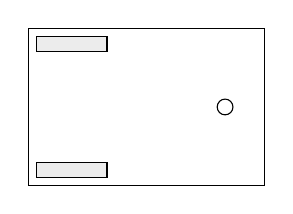
\begin{tikzpicture}
\draw (0,0) rectangle (3,2);
\draw[fill=gray!15] (0.1,0.1) rectangle (1,0.3);
\draw[fill=gray!15] (0.1,1.9) rectangle (1,1.7);
\draw (2.5,1) circle (0.1cm);
\end{tikzpicture}
\caption{Geometrical arrangement shows two standard wheels, each driven by a separate motor, in a differential drive configuration. A passive omnidirectional wheel is mounted at the opposite end of the chassis.}
\end{figure}
\end{minipage}
\end{frame}

%------------------------------------------------

\begin{frame}
\frametitle{Hardware: How does the robot sense the world?}
Two main devices used to sense the environment in the field of mobile robotics:\\
\vspace{0.25cm}
\begin{minipage}[t]{0.45\textwidth}
\begin{figure}
\centering
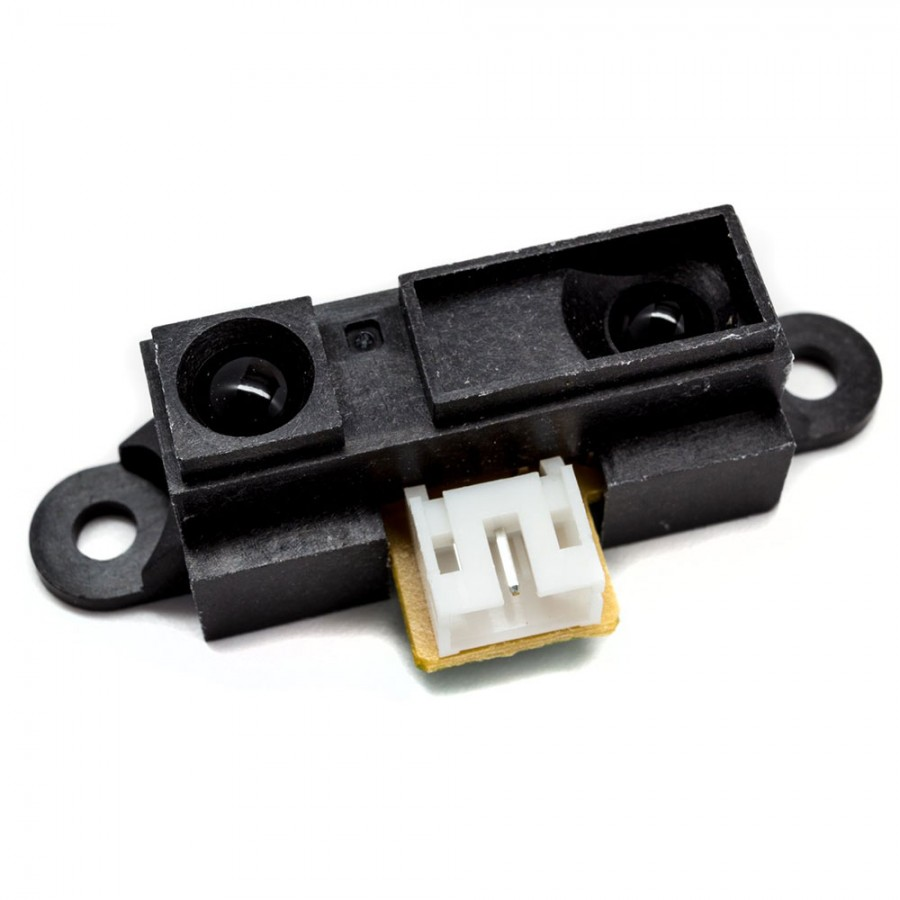
\includegraphics[height=3cm]{sharp_sensor}
\caption{One-dimensional Infra-red ranging sensor}
\end{figure}
\vspace{-1cm}
\begin{figure}
\centering
\includegraphics[height=1cm]{green_tick}
\end{figure}
\end{minipage}
\hspace{1cm}
\begin{minipage}[t]{0.45\textwidth}
\begin{figure}
\centering
\includegraphics[height=3cm]{ultrasonic}
\caption{Ultrasonic time of flight ranging sensor}
\end{figure}
\vspace{-0.6cm}
\begin{figure}
\centering
\includegraphics[height=1cm]{red_cross}
\end{figure}
\end{minipage}
\end{frame}


%------------------------------------------------
\begin{frame}
\frametitle{Hardware: How does the robot sense the world?}
The two main sensors for obtaining odometry (i.e. the robot tracking it's position) are:\\
\vspace{0.5cm}
\begin{minipage}[t]{0.45\textwidth}
\begin{figure}
\centering
\frame{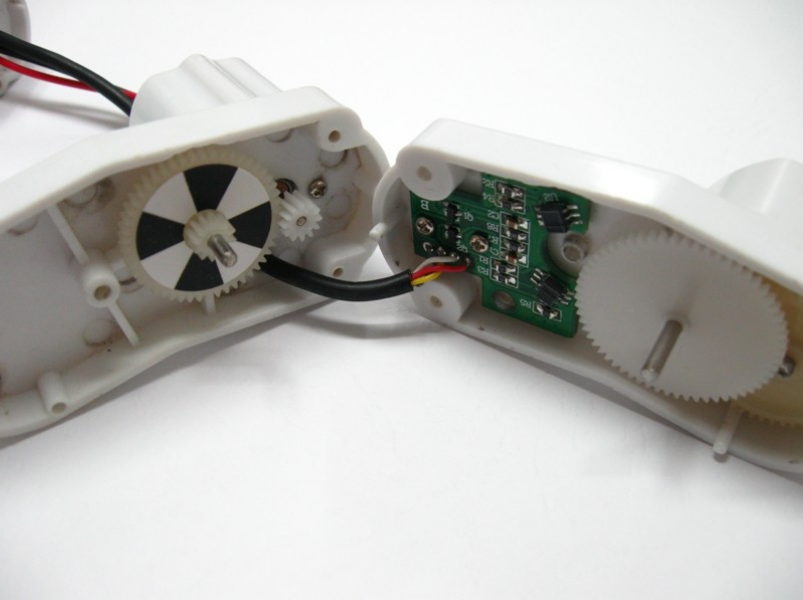
\includegraphics[height=3cm]{optical_encoder_actual}}
\caption{Quadrature optical rotary encoder}
\end{figure}
\vspace{-0.5cm}
\begin{figure}
\centering
\includegraphics[height=1cm]{green_tick}
\end{figure}
\end{minipage}
\hspace{1cm}
\begin{minipage}[t]{0.45\textwidth}
\begin{figure}
\centering
\includegraphics[height=3cm]{imu}
\caption{Inertial measurement unit}
\end{figure}
\vspace{-0.6cm}
\begin{figure}
\centering
\includegraphics[height=1cm]{red_cross}
\end{figure}
\end{minipage}
\end{frame}

%------------------------------------------------

\begin{frame}
\frametitle{Hardware: How does the robot sense the world?}
Additional sensor used to detect the red exit area:
\begin{figure}
\centering
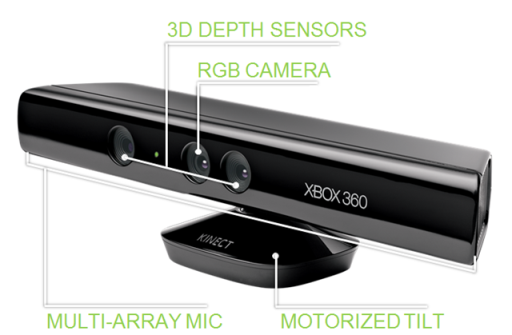
\includegraphics[height=6cm]{kinect}
\end{figure}
\end{frame}

%------------------------------------------------

\begin{frame}
\frametitle{Hardware: Powering the Robot}
\begin{itemize}
\item Two power sources were used to power the robot.
\item DC motors are noisy and can interfere with the performance of the myRIO 
\end{itemize}
\begin{minipage}{0.45\textwidth}
\begin{figure}
\centering
\includegraphics[height=4cm]{aa_cell}
\caption{6 $\times$ 1.5V AA cells were used in series to provide 9V supply to motors}
\end{figure}
\end{minipage}
\hspace{1cm}
\begin{minipage}{0.45\textwidth}
\begin{figure}
\includegraphics[height=4cm]{12_volt_battery}
\caption{12V 4.5Ah battery was used to supply power to myRio and Microsoft Kinect}
\end{figure}
\end{minipage}
\end{frame}

%------------------------------------------------

\begin{frame}
\frametitle{Robot Movement: What are the choices?}
Now that the robot has a physical body, can sense the world, and is powered, how should it move from one point in the world to another? There are two main choices:\\
\vspace{0.25cm}
\begin{minipage}[t]{0.45\textwidth}
\textbf{Stochastic Movement}\\
\begin{figure}
\centering
\frame{\includegraphics[height=3cm]{stochastic}}
\caption{Stochastic movement sees the robot bounce around the environment in a randomised fashion.}
\end{figure}
\end{minipage}
\hspace{1cm}
\begin{minipage}[t]{0.45\textwidth}
\textbf{Controlled Movement}\\
\begin{figure}
\centering
\includegraphics[height=2.5cm]{pid}
\caption{Controlled movement can move a robot to a desired location, but requires more sophisticated technology, like PID controllers.}
\end{figure}
\end{minipage}
\end{frame}

%------------------------------------------------

\begin{frame}
\frametitle{Robot Control: Go To Goal}
A picture of how the pid controller works.
\begin{figure}
\centering
\includegraphics[height=6.5cm]{comp_diagram}
\end{figure}
\end{frame}

%------------------------------------------------

\begin{frame}
\frametitle{Robot Control: Go To Goal}
A picture of how the pid controller works.

\begin{figure}
\begin{overpic}[height=6.5cm]{comp_diagram}
 \put (20,40) {\huge \color{red}\textbf{JUST KIDDING}}
\end{overpic}
\end{figure}
\end{frame}

%------------------------------------------------

\begin{frame}
\frametitle{Robot Control: Go To Goal}
\begin{center}
\includemedia[
  activate=pageopen,
  width=264pt,height=198pt,
  addresource=gtgdemo.mp4,
  flashvars={%
     source=gtgdemo.mp4% same path as in addresource!
%   &autoPlay=true%    % optional configuration
%   &loop=true%        % variables
  }  
]{}{VPlayer.swf}
\end{center}
\end{frame}

%------------------------------------------------

\begin{frame}
\frametitle{Robot Control: Go To Goal}
\begin{center}
\includemedia[
  activate=pageopen,
  width=264pt,height=198pt,
  addresource=pidgtg.mp4,
  flashvars={%
     source=pidgtg.mp4% same path as in addresource!
%   &autoPlay=true%    % optional configuration
%   &loop=true%        % variables
  }  
]{}{VPlayer.swf}
\end{center}
\end{frame}

%------------------------------------------------

\begin{frame}
\frametitle{Robot Control: Avoiding Obstacles}
\begin{minipage}{0.45\textwidth}
\begin{itemize}
\item How can we create an input signal which will use the PID controller to avoid obstacles? \textbf{Vectors} \ensuremath\heartsuit
\vspace{1cm}
\item A vector from the center of the robot is made to the sensing location for each sensor.
\vspace{1cm}
\item The sum of these vectors is used to create an input reference for the PID
\end{itemize}
\end{minipage}
\hspace{1cm}
\begin{minipage}{0.45\textwidth}
\begin{figure}
\centering
\frame{\includegraphics[height=5cm]{obstacle_avoidance}}
\caption{Simulated mobile robot with 5 sensors, near an obstacle}
\end{figure}
\end{minipage}
\end{frame}

%------------------------------------------------

\begin{frame}
\frametitle{Robot Control: Avoiding Obstacles}
\begin{center}
\includemedia[
  activate=pageopen,
  width=264pt,height=198pt,
  addresource=oasim.mp4,
  flashvars={%
     source=oasim.mp4% same path as in addresource!
%   &autoPlay=true%    % optional configuration
%   &loop=true%        % variables
  }  
]{}{VPlayer.swf}
\end{center}
\end{frame}

%------------------------------------------------

\begin{frame}
\frametitle{The Story So Far...}
The robot now has:\\
\begin{itemize}
\item A body, sensors, and power
\vspace{0.25cm}
\item The ability to move to a desired location in the environment
\vspace{0.25cm}
\item The ability to avoid obstacles
\end{itemize}
\vspace{1cm}
\begin{center}
\huge\textit{Now what?}
\end{center}
\end{frame}

%------------------------------------------------

\begin{frame}
\frametitle{Mapping the World: Occupancy Grids}
One of the main approaches to mapping the world is to discretise the environment - this type of map is called an occupancy grid.
\begin{figure}
\centering
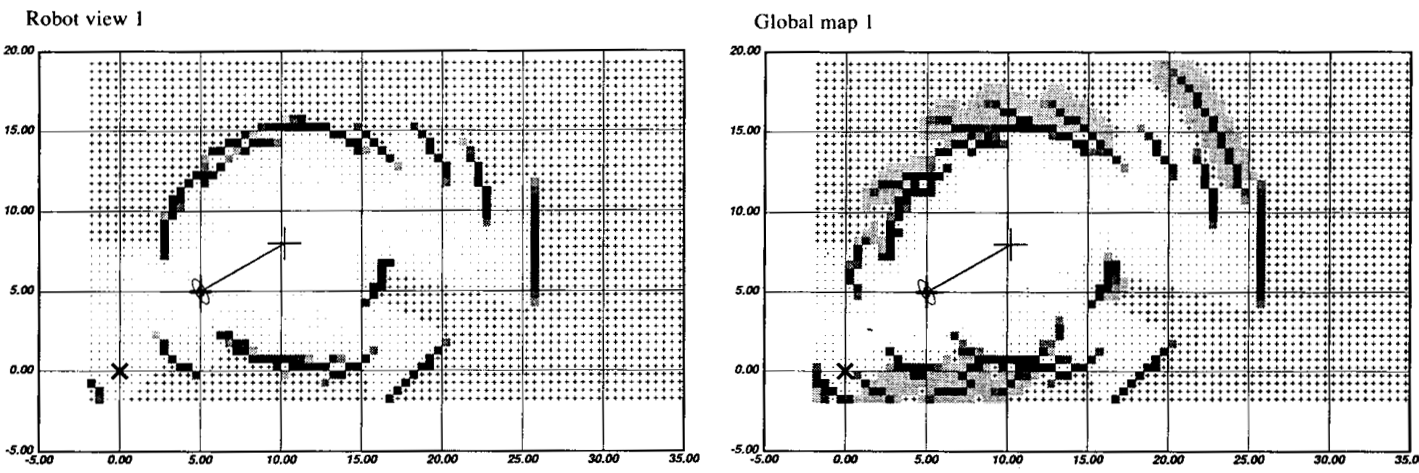
\includegraphics[height=5cm]{occupancy_grid}
\caption{Image taken from Alberto Elfes’ 1989 paper \textit{Using Occupancy Grids for Mobile Robot Perception and Navigation}}
\end{figure}
\end{frame}

%------------------------------------------------

\begin{frame}
\frametitle{Mapping the World: Uncovering the Map}
\begin{center}
\includemedia[
  activate=pageopen,
  width=264pt,height=198pt,
  addresource=occgrid.mp4,
  flashvars={%
     source=occgrid.mp4% same path as in addresource!
%   &autoPlay=true%    % optional configuration
%   &loop=true%        % variables
  }  
]{}{VPlayer.swf}
\end{center}
\end{frame}

%------------------------------------------------

\begin{frame}
\frametitle{Mapping the World: Locating Objects}
\begin{center}
\includemedia[
  activate=pageopen,
  width=264pt,height=198pt,
  addresource=objectdetect.mp4,
  flashvars={%
     source=objectdetect.mp4% same path as in addresource!
%   &autoPlay=true%    % optional configuration
%   &loop=true%        % variables
  }  
]{}{VPlayer.swf}
\end{center}
\end{frame}

%------------------------------------------------

\begin{frame}
\frametitle{Strategic Navigation: Where Should We Go?}
\begin{center}
\footnotesize\textit{Given what you know about the world, where should you move to gain as much new information as possible?}
\end{center}
\begin{minipage}{0.45\textwidth}
\begin{figure}
\centering
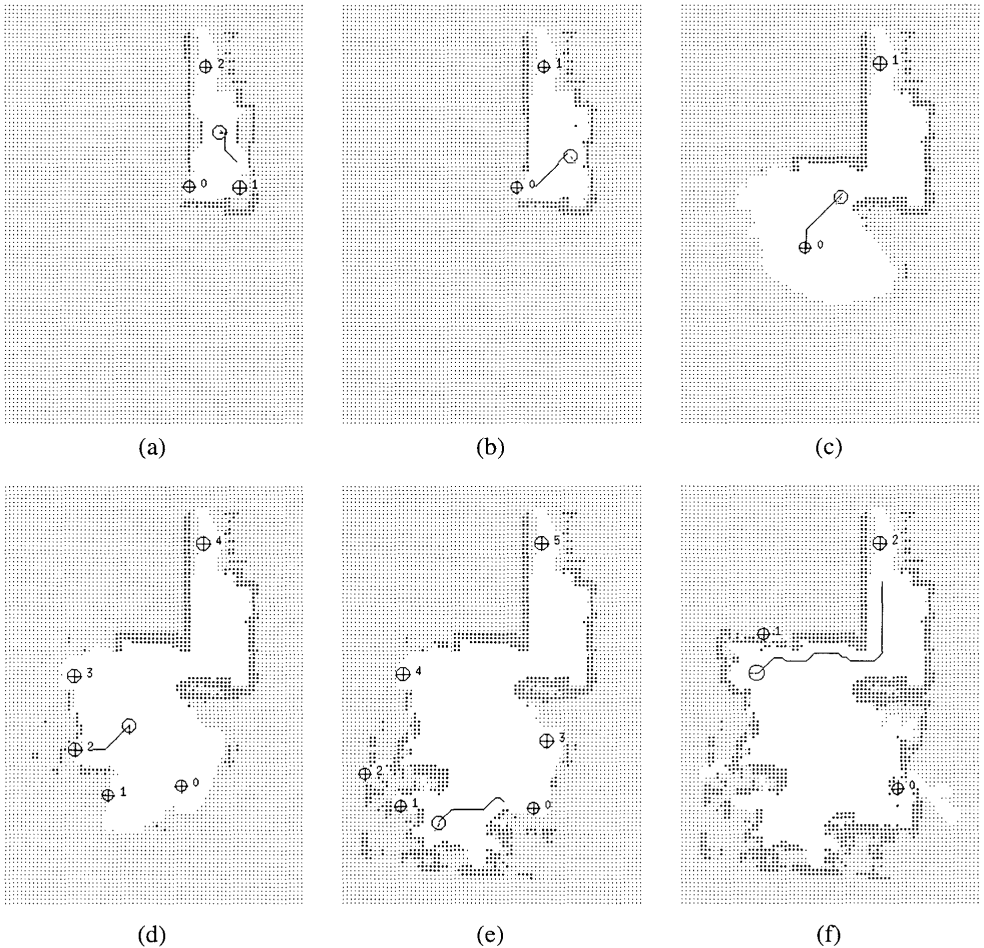
\includegraphics[height=6cm]{frontier_exploration}
\end{figure}
\end{minipage}
\begin{minipage}{0.45\textwidth}
\begin{itemize}
\item Frontier exploration finds the pixels which form a boundary between the explored and unexplored regions
\vspace{0.35cm}
\item In our implementation, once the PID reaches its goal, it asks the strategic planner for another navigation point.
\vspace{0.35cm}
\item The navigation point is the mean coordinate values of a subset of the frontier points.
\end{itemize}
\end{minipage}
\end{frame}

%------------------------------------------------

\begin{frame}
\frametitle{Strategic Navigation: Where Should We Go?}
\begin{center}
\includemedia[
  activate=pageopen,
  width=264pt,height=198pt,
  addresource=explorationstrategy.mp4,
  flashvars={%
     source=explorationstrategy.mp4% same path as in addresource!
%   &autoPlay=true%    % optional configuration
%   &loop=true%        % variables
  }  
]{}{VPlayer.swf}
\end{center}
\end{frame}

%------------------------------------------------

\begin{frame}
\frametitle{Strategic Navigation: Are We There Yet?}
To detect the red panel, an optical image was taken every 200 milliseconds and a colour threshold filter was used to extract a binary threshold image of red objects.\\
\vspace{0.25cm}
\begin{minipage}{0.45\textwidth}
\begin{figure}
\centering
\frame{\includegraphics[height=4cm]{rgb_color_space}}
\caption{The RGB colour space is comprised of Red, Green, and Blue channels with values ranging from 0 to 255}
\end{figure}
\end{minipage}
\hspace{1cm}
\begin{minipage}{0.45\textwidth}
\begin{figure}
\centering
\frame{\includegraphics[height=4cm]{color_detection_blue_version}}
\caption{Colour detection relies on filtering out image pixels which do no fall within specified ranges for the R, G, and B channels.}
\end{figure}
\end{minipage}
\end{frame}

%------------------------------------------------

\begin{frame}
\frametitle{Strategic Navigation: Are We There Yet?}
\begin{center}
\includemedia[
  activate=pageopen,
  width=264pt,height=198pt,
  addresource=kinectdemo.mp4,
  flashvars={%
     source=kinectdemo.mp4% same path as in addresource!
%   &autoPlay=true%    % optional configuration
%   &loop=true%        % variables
  }  
]{}{VPlayer.swf}
\end{center}
\end{frame}

%------------------------------------------------

\begin{frame}
\frametitle{Completed Package}
\begin{minipage}{0.45\textwidth}
\begin{figure}
\centering
\frame{\includegraphics[height=4cm]{complete_robot}}
\caption{The completed robot with the Microsoft Kinect attached.}
\end{figure}
\end{minipage}
\hspace{0.25cm}
\begin{minipage}{0.45\textwidth}
\footnotesize The complete package loops the following steps until the red panel is detected:
\begin{enumerate}
\item Look at the map and find the set of frontier pixels
\vspace{0.1cm}
\item Choose a subset of the frontier pixels randomly to determine a navigation point.
\vspace{0.1cm}
\item Pass the navigation point to the PID controller.
\vspace{0.1cm}
\item PID executes until robot is within 5cm of the desired location (or 10 seconds elapses).
\item If the robot encounters an obstacle it switches PID reference set point to avoid obstacles until the obstacle is cleared. The robot updates the map during this entire time.
\end{enumerate}
\end{minipage}
\end{frame}

%----------------------------------------------------------------------------------------

\end{document} 